\subsection{Valve Closing Simulations}



For $\alpha = 0.1$ and $\beta = 1$, the simulation results are shown below

\begin{figure}[!ht]
    \centering
    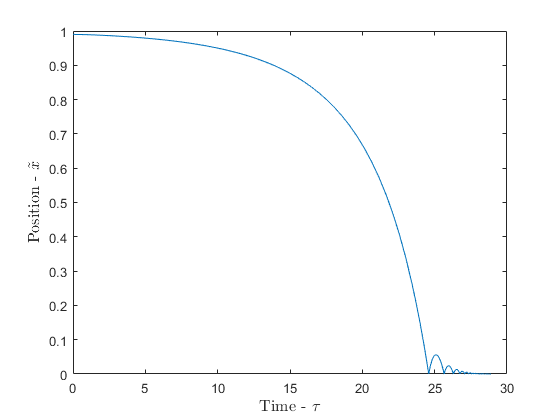
\includegraphics[width=0.7\textwidth]{Figures/Example/PositionTimeTrajectory.png}
    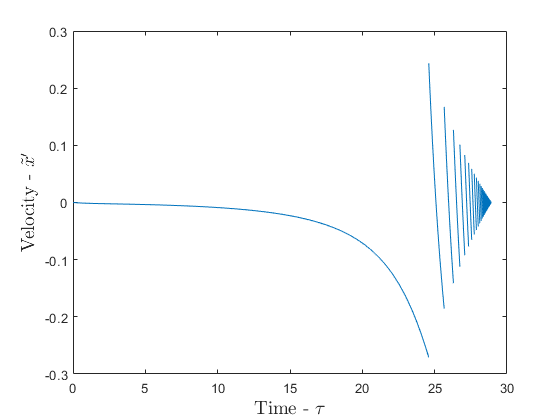
\includegraphics[width=0.49\textwidth]{Figures/Example/VelocityTimeTrajectory.png}
    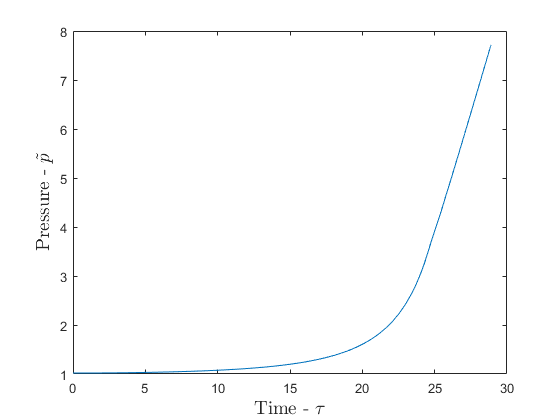
\includegraphics[width=0.49\textwidth]{Figures/Example/PressureTimeTrajectory.png}
    \caption{Caption}
    \label{fig:TimeTrajec}
\end{figure}

% % Example Trajectory in Phase Portrait - PROBABLY NOT WORTH USING
% \begin{figure}[!ht]
%     \centering
%     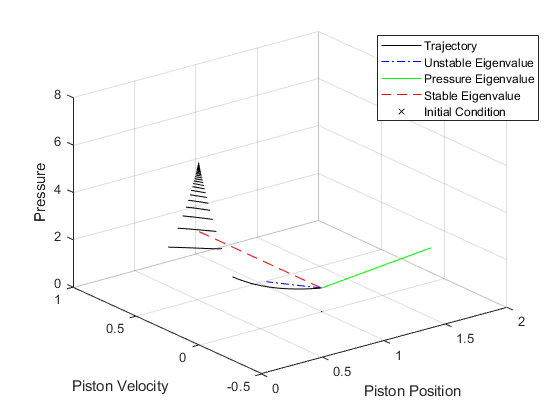
\includegraphics[width=0.49\textwidth]{Figures/Example/PhasePotrait3D.png}
%     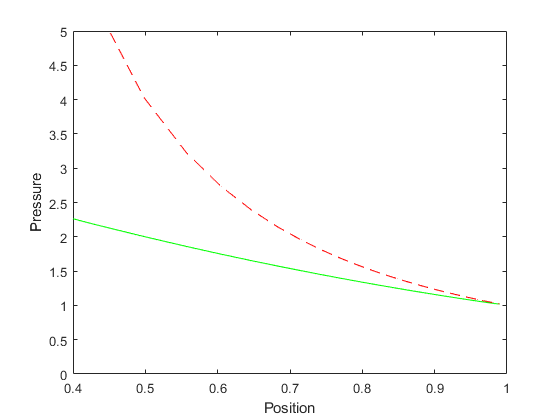
\includegraphics[width=0.49\textwidth]{Figures/Example/PressurePositionPhasePotrait2D.png}
%     \caption{Caption}
%     \label{fig:ExamplePhase}
% \end{figure}

% % Example Trajectory in eigenvector projected Phase Portrait - DO NOT USE
% \begin{figure}[!ht]
%     \centering
%     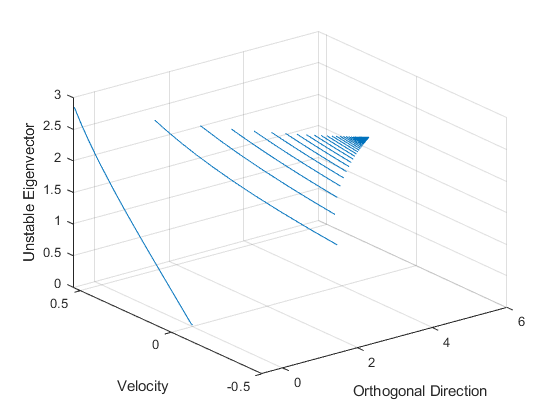
\includegraphics[width=0.7\textwidth]{Figures/Example/EigenvectorPhasePotrait3D.png}
%     \caption{Caption}
%     \label{fig:EigPhase}
% \end{figure}

% % Example Trajectory of eigenvector space in 2D Phase and 1D unstable trajectory - DO NOT USE
% \begin{figure}[!ht]
%     \centering
%     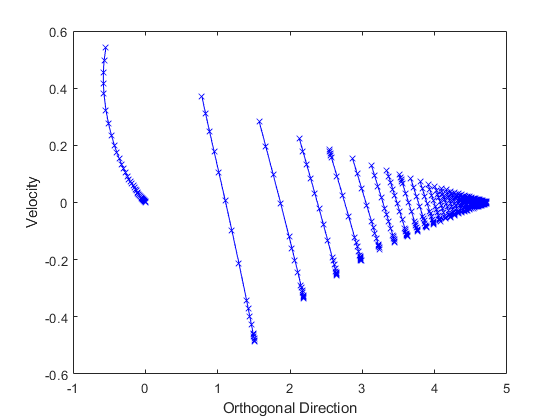
\includegraphics[width=0.49\textwidth]{Figures/Example/PhasePotrait2D.png}
%     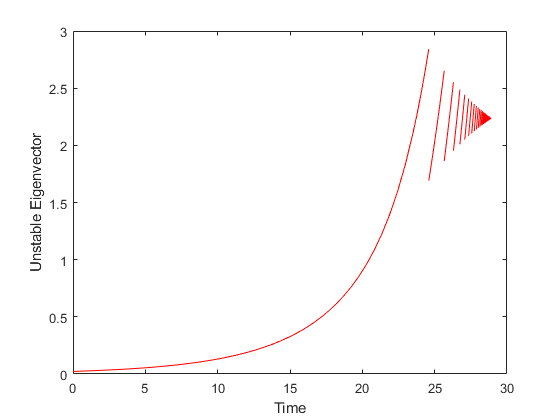
\includegraphics[width=0.49\textwidth]{Figures/Example/UnstableEigenvectorTrajectory.png}
%     \caption{Caption}
%     \label{fig:EigenvectorPhase}
% \end{figure}

\newpage
\subsection{Low flow rates}

For low flow rates, $\dot{m}_{in} \rightarrow 0$, meaning that $\alpha \rightarrow 0$ and $\beta \rightarrow \infty$. Considering only the limit as $\alpha \rightarrow 0$, the eigenvalues and eigenvectors are

\begin{equation*}
\begin{split}
    % eigenvalues
    \lambda_1 = - \frac{1}{2}\beta \, , \quad
    \lambda_2 = -1 \, , \quad
    \lambda_3 = 0 \\
    % eigenvectors
    v_1 = \begin{pmatrix}
    0 \\ 0 \\ 1
    \end{pmatrix} \qquad
    v_2 = \begin{pmatrix}
    \frac{2 - \beta}{2\beta} \\ \frac{\beta - 2}{2\beta} \\ 1
    \end{pmatrix} \qquad
    v_3 = \begin{pmatrix}
    - \frac{1}{2} \\ 0 \\ 1
    \end{pmatrix}
\end{split}
\end{equation*}

The dynamics approach the equation

\begin{equation*}
    1 - x \sqrt{p} = 0 \, .
\end{equation*}

% Simulation results support this. 
% 
% % 2D Phase Portrait showing low flow rate trajectory close to manifold - PROBABLY DO NOT (TOO SIMILAR TO BELOW)
% \begin{figure}[ht]
%     \centering
%     \begin{subfigure}{0.49\textwidth}
%     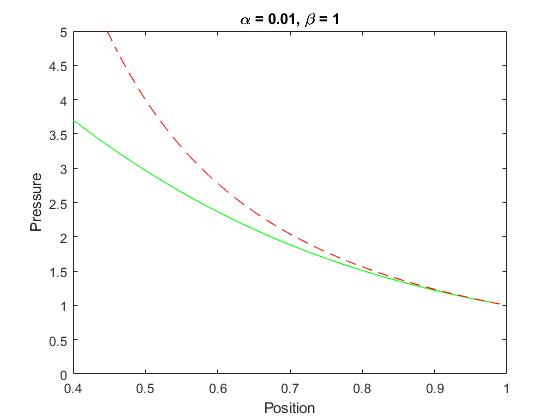
\includegraphics[width=\textwidth]{Figures/LowFlow/b=1.png}
%     \caption{$\alpha = 0.01, \, \beta = 1$}
% %    \label{fig:1}
%     \end{subfigure}
%     \begin{subfigure}{0.49\textwidth}
%     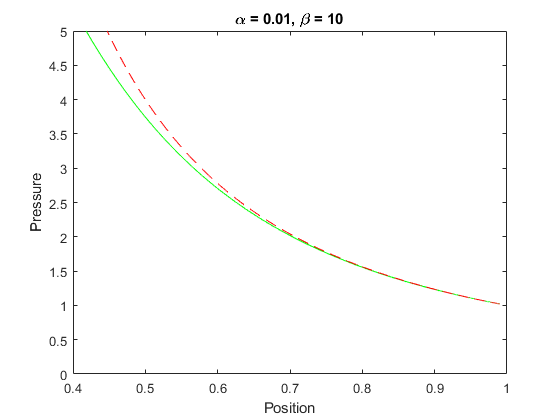
\includegraphics[width=\textwidth]{Figures/LowFlow/b=10.png}
%     \caption{$\alpha = 0.01, \, \beta = 10$}
% %    \label{fig:2}
%     \end{subfigure}
% %    \label{3}
% %    \caption{}
% \end{figure}

The three dimensional phase portrait in Position-Velocity-Pressure phase space can be seen below.

\begin{figure}[ht]
    \centering
    \begin{subfigure}{0.49\textwidth}
    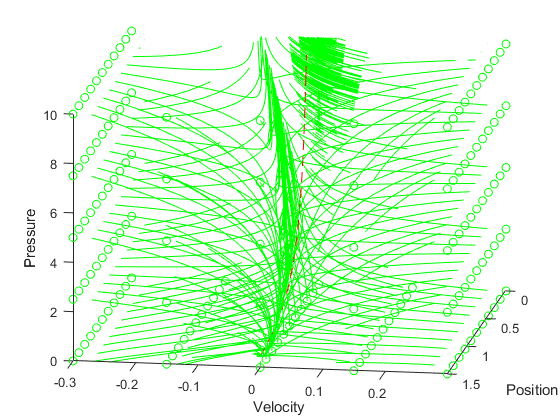
\includegraphics[width=\textwidth]{Figures/LowFlow/3DPhase-b=1.png}
    \caption{$\alpha = 0.01, \, \beta = 1$}
%    \label{fig:1}
    \end{subfigure}
    \begin{subfigure}{0.49\textwidth}
    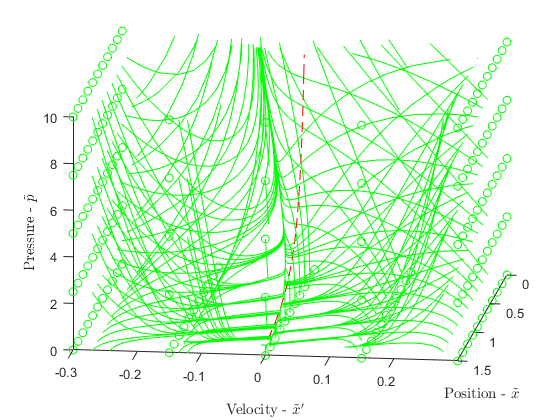
\includegraphics[width=\textwidth]{Figures/LowFlow/3DPhase-b=10.png}
    \caption{$\alpha = 0.01, \, \beta = 10$}
%    \label{fig:2}
    \end{subfigure}
%    \label{3}
%    \caption{}
\end{figure}



The phase portrait in Position-Pressure space can be seen below

\begin{figure}[ht]
    \centering
    \begin{subfigure}{0.49\textwidth}
    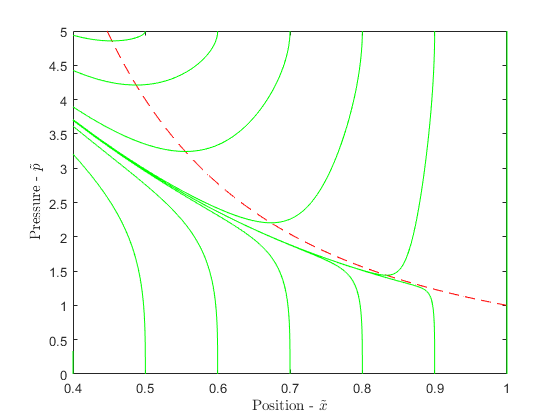
\includegraphics[width=\textwidth]{Figures/LowFlow/PhasePortrait-b=1.png}
    \caption{$\alpha = 0.01, \, \beta = 1$}
%    \label{fig:1}
    \end{subfigure}
    \begin{subfigure}{0.49\textwidth}
    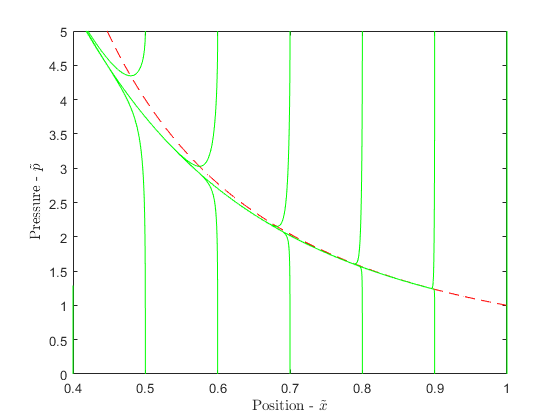
\includegraphics[width=\textwidth]{Figures/LowFlow/PhasePortrait-b=10.png}
    \caption{$\alpha = 0.01, \, \beta = 10$}
%    \label{fig:2}
    \end{subfigure}
%    \label{3}
%    \caption{}
\end{figure}